\chapter{Jacobi Fields}
\label{chap:jacobi}
\vspace*{-0.9cm}

% \startcontents[chapters]
% \printcontents[chapters]{}{3}{}

\section{The Jacobi Equation}
\label{sec:jacobieq}
In this section we focus on semi-Riemannian manifolds.
\begin{definition}[Variation through Geodesics]
    Let $(M,g)$ be semi-Riemannian and $\gamma: I \to M$ be a geodesic. If $K$ is another interval and \[
    \Gamma: K \times I \to M
    \] is a variation of $\gamma$ such that $\gamma_s: I \to M$ is a geodesic for all $s \in K$, we call $\Gamma$ a \textbf{variation through geodesics}. 
\end{definition}

Variation through geodesics give rise to several particular vector fields: The \emph{variational field} of $\Gamma$ is a vector field $J \in \mathfrak{X}(\Gamma)$ defined as \[
    J(t):=\left.\frac{\partial}{\partial s}\right|_{s=0} \Gamma (s,t)
.\] Furthermore, we define two accessory vector fields 
\[    T(s,t) := \frac{\partial \Gamma}{\partial t} \]
\[S(s,t)  := \frac{\partial \Gamma}{\partial s} \]
which will be useful.
\begin{lemma}[Symmetry Lemma]
    \label{lem:symmlemm}
    Let $\Gamma: K \times I \to M$ be a smooth family of curves. Then we have \[
        \nabla_{\frac{d}{ds}} T = \nabla_{\frac{d}{dt}}S
    .\] 
\end{lemma}
\begin{proof}
    Take local coordinates $(x^i)$ on some coordinate neighbourhood and write $\Gamma(s,t)=(\gamma^1(s,t), \dots, \gamma^n(s,t))$. We have $S = \frac{\partial \gamma^k}{\partial s} \partial_k$ and $T= \frac{\partial \gamma^k}{\partial t} \partial_k$. Calculating the left side directly yields:
    \begin{align*}
\nabla_{\frac{d}{ds}} T &= \nabla_{\frac{d}{ds}}\left( \frac{\partial \gamma^k}{\partial s} \partial_k \right) = \frac{\partial^2 \gamma^k}{\partial t \partial s} \partial_k + \frac{\partial \gamma^i}{\partial t} \frac{\partial \gamma^j}{\partial s} \nabla_{\partial_j}\partial_i \\
                        &= \left(  \frac{\partial^2 \gamma^k}{\partial t \partial s} + \frac{\partial \gamma^i}{\partial t} \frac{\partial \gamma^j}{\partial s} \Gamma_{ji}^k \right) \partial_k
    \end{align*}
    Exchanging $i \leftrightarrow j$ and using the symmetry $\Gamma_{ij}^k=\Gamma_{ji}^k$ yields the desired identity.
\end{proof}
\begin{lemma}[Curvature Lemma]
    \label{lem:curvlem}
    Let $(M,g)$ be semi-Riemannian and $\Gamma: K \times I \to M$ be a smooth family of curves. Then for any $V \in \mathfrak{X}(\Gamma)$, we have \[
        \nabla_{\frac{d}{ds}} \nabla_{\frac{d}{dt}} V - \nabla_{\frac{d}{dt}} \nabla_{\frac{d}{ds}}V = R(S, T)V
    .\] 
\end{lemma}
\begin{proof}
    Take local coodinates $(x^i)$ and write $\Gamma(s,t)=(\gamma^1(s,t), \dots, \gamma^n(s,t))$ as well as $V=V^i\partial_i$. We calculate the two left derivatives explicitly:
    \[
        \nabla_{\frac{d}{dt}}V=\frac{\partial V^i}{dt}\partial_i + V^i \nabla_{\frac{d}{dt}} \partial_i
    \] and \[
    \nabla_{\frac{d}{ds}} \nabla_{\frac{d}{dt}} V= \left( \frac{\partial^2 V^i}{\partial s \partial t} + \frac{\partial V^i}{\partial t} \nabla_{\frac{d}{ds}} + \frac{\partial V^i}{\partial s} \nabla_{\frac{d}{dt}} + V^i \nabla_{\frac{d}{ds}} \nabla_{\frac{d}{dt}} \right) \partial_i
    .\] 
Exchanging $s \leftrightarrow t$ yields $\nabla_{\frac{d}{dt}} \nabla_{\frac{d}{ds}} V$ and we see immediately that after subtraction, only the rightmost term remains: \[
\left( \nabla_{\frac{d}{ds}} \nabla_{\frac{d}{dt}} - \nabla_{\frac{d}{dt}} \nabla_{\frac{d}{ds}}\right) V = V^i \left(\nabla_{\frac{d}{ds}} \nabla_{\frac{d}{dt}} - \nabla_{\frac{d}{dt}} \nabla_{\frac{d}{ds}} \right) \partial_i
.\] 
Extending $\partial_i$ and the covariant derivative, we can calculate:
\[
    \nabla_{\frac{d}{ds}} \nabla_{\frac{d}{dt}} \partial_i = \nabla_{\frac{d}{ds}} \left(  \frac{\partial \gamma^j}{\partial t} \nabla_{\partial_j}\partial_i\right)= \frac{\partial^2 \gamma^j}{\partial s \partial t} \nabla_{\partial_j} \partial_i + \frac{\partial \gamma^j}{\partial t} \frac{\partial \gamma^k}{\partial s} \nabla_{\partial_k} \nabla_{\partial_j}\partial_i
\] and analogously \[
    \nabla_{\frac{d}{dt}} \nabla_{\frac{d}{ds}} \partial_i = \frac{\partial^2 \gamma^j}{\partial t \partial s} \nabla_{\partial_j} \partial_i + \frac{\partial \gamma^j}{\partial s} \frac{\partial \gamma^k}{\partial t} \nabla_{\partial_k} \nabla_{\partial_j}\partial_i
.\] 
Exchanging $j \leftrightarrow k$ and subtracting cancels out the left term and we obtain: \[
    \nabla_{\frac{d}{ds}} \nabla_{\frac{d}{dt}} \partial_i -     \nabla_{\frac{d}{dt}} \nabla_{\frac{d}{ds}} \partial_i \partial_i = \frac{\partial \gamma^j}{\partial t} \frac{\partial \gamma^k}{\partial s} (\nabla_{\partial_k} \nabla_{\partial_j}-\nabla_{\partial_j}\nabla_{\partial_k}) \partial_i = R(S,T)\partial_i
.\] 
\end{proof}
We are now ready to consider the main theorem of this section:
\begin{theorem}[Jacobi Equation]
    Let $(M,g)$ be semi-Riemannian, $\gamma: I \to M$ be a geodesic and $\Gamma: K \times I \to M$ be a variation of $\gamma$ through geodesics with variational field $J$. Then $J$ satisfies the \textbf{Jacobi Equation}: 
    \begin{equation}
        \nabla_{\frac{d}{dt}}^2 J + R(J,\dot{\gamma})\dot{\gamma}=0.
    \end{equation}
\end{theorem}
\begin{proof}
    The fact that $\Gamma$ is a variation through geodesics tells us that $\nabla_{\frac{d}{dt}}T \equiv 0$. Dervating once more yields $\nabla_{\frac{d}{ds}}\nabla_{\frac{d}{dt}}\equiv 0$. By the curvature and the symmetry lemma, we have \[
        \nabla_{\frac{d}{ds}} \nabla_{\frac{d}{dt}} T = \nabla_{\frac{d}{dt}} \nabla_{\frac{d}{ds}} T + R(S,T)T = \nabla_{\frac{d}{dt}}^2 S + R(S,T)T
    .\] 
At $s=0$, we have $S(0,t)=\partial_s \Gamma_s(t)= J(t)$ and $T(0,t)=\partial_t \Gamma_0 (t)=\dot{\gamma}(t)$ as claimed.
\end{proof}
\begin{prop}[Existence and Uniqueness]
Let $(M,g)$ be a SRMF, $\gamma: I \to M$ be a geodesic, $t_0 \in I$ and $p:=\gamma(t_0)$. For all $v,w \in T_pM$, there is a unique Jacobi field $J$ along $\gamma$ satisfying the initial data \[
        J(t_0) = v, \, \nabla_{\frac{d}{dt}} J(t_0)=w
    .\] 
\end{prop}
\begin{proof}
    Take $J \in \mathfrak{X}(\gamma)$ and choose a parallel ONF $(E_i)$. We write $v = v^iE_i(t_0)$, $w = w^iE_i(t_0)$, $\dot{\gamma}(t)=\gamma^i(t)E_i(t)$ and $J=J^i(t)E_i(t)$. The Jacobi equation holds if and only if the following equation is satisfied:
    \marginnote{Note that all terms of the form $\nabla_{\frac{d}{dt}} E_i$ in the left term vanish as the ONF is parallel w.r.t. $\nabla$.}
    \begin{align*}
        0 &= \nabla_{\frac{d}{dt}}^2 J + R(J, \dot{\gamma})\dot{\gamma} = \nabla_{\frac{d}{dt}}^2 (J^iE_i)  + R(J^j E_j, \dot{\gamma}^kE_k)\dot{\gamma}^lE_l\\
          &= \ddot{J}^iE_i + J^j \dot{\gamma}^k \dot{\gamma}^l R(E_j,E_k)E_l 
    \end{align*}
    This yields a second-order system of $n$ equations \[
        \frac{d^2 J^i(t)}{dt^2} = - \dot{J}^j  (t) \dot{\gamma}^k(t)\dot{\gamma}^l(t) R^i_{jkl}
    .\] Substituting $W^i(t):=\dot{J}^i(t)$, this reduces to $2n$ first-order equations. The existence and uniqueness theorem of ODEs on manifolds thus guarantees that the claim holds.
\end{proof}
\begin{definition}[Jacobi Field]
    Let $(M,g)$ be a SRMF and $\gamma: I \to M$ be a geodesic. We call a vector field $J \in \mathfrak{X}(\gamma)$ a \textbf{Jacobi field} if it satiesfies the Jacobi equation. The space $\mathfrak{J}(\gamma) \subseteq \mathfrak{X}(\gamma)$ denotes the space of all Jacobi fields along $\gamma$.
\end{definition}
\begin{corollary}
    \label{cor:jsubspace}
   Let $(M,g)$ be an $n$-dimensional SRMF and $\gamma: I \to M$ be any geodesic. Then $\mathfrak{J}(\gamma)$ is a $2n$-dimensional linear subspace of $\mathfrak{X}(\gamma)$.
\end{corollary}
\begin{proof}
    Linearity of the Jacobi equation guarantees that $\mathfrak{J}(\gamma)$ is linear. Fixing some $p=\gamma(t_0)$, we have an isomorphism $\mathfrak{J}(\gamma) \cong T_p M \oplus T_p M$ given by the previous preposition as $J \mapsto (J(t_0), \nabla_{\frac{d}{dt}} J(t_0))$.
\end{proof}
\begin{prop}
    Let $(M,g)$ be a SRMF and $\gamma: I \to M$ be a geodesic. If either 
    \begin{enumerate}[(i)]
        \item $M$ is complete, or
        \item $I$ is compact
    \end{enumerate}
    then every Jacobi field along $\gamma$ is the variation field of some variation of $\gamma$ though geodesics.
\end{prop}
\begin{proof}
    \marginnote{The idea is the following: We define a small curve through a starting point on $\gamma$ and use the assumptions to guarantee that (after eventually contracting the domain) $\exp$ can be used to define a variation through geodesics. After that, we use uniqueness of Jacobi fields to show that the variational vector field of this constructed variation has to agree with $J$.}
    Let $J \in \mathfrak{J}(\gamma)$. By translating, we can assume $0 \in I$ and set $p:=\gamma(0)$, $v:=\dot{\gamma}(0)$. This means we can write $\gamma(t)=\exp_p(tv)$ for all $t \in I$. By construction of the tangent space, there is a small open interval $(-\epsilon, \epsilon)$ and a smooth curve $\sigma: (- \epsilon, \epsilon) \to M$ satisfying \[
        \sigma(0)=p, \, \dot{\sigma}(0)=J(0)
    .\] Choose a vector field $V \in \mathfrak{X}(\sigma)$ with data \[
    V(0)=w \, \nabla_{\frac{d}{ds}}V(0)=\nabla_{\frac{d}{dt}}J(0)
    .\] We want to define a variation through geodesics by 
    \begin{equation}
    \label{eq:jacobivar}
        \Gamma(s,t):=\exp_{\sigma(s)}(tV(s)).
    \end{equation}
    If $M$ is geodesically complete, we can always define $\Gamma$ on $(-\epsilon, \epsilon) \times I$. If $I$ is compact, we can use that $\mathcal{E}_p$ is open and contains the compactum $\{(p,tv)\in TM \mid t\in I\}$. Therefore, we find some $\delta >0$ such that $\Gamma$ is definable on $(-\delta, \delta) \times M$. \\
Evaluating at $s=0$ yields \[
    \Gamma_0(t)= \exp_{\sigma(0)}(tV(0))=\exp_p(tv)=\gamma(t),
\] which tells us that $\Gamma$ is indeed a variation of $\gamma$: By definition of $\exp$, it is also a variation thorugh geodesics with variational field $W(t):=\frac{\partial \Gamma}{\partial s}(0,t) \in \mathfrak{J}(\gamma)$. \\
Now we match initial data:
\begin{enumerate}
    \item $W(0)=\frac{\partial}{\partial s} \Gamma(0,0) = \dot{\sigma}(0)=J(0)$
    \item We have $\frac{\partial}{\partial t}\Gamma_s(0) = V(s)\exp(0)=V(s)$. By applying the symmetry lemma, we obtain: \[
            \nabla_{\frac{d}{dt}}W(0)=\nabla_{\frac{d}{dt}} \frac{\partial}{\partial s} \Gamma(0,0) = \nabla_{\frac{d}{ds}} \frac{\partial}{\partial t}\Gamma(0,0) = \nabla_{\frac{d}{ds}}V(0)=\nabla_{\frac{d}{dt}}J(0)
    .\] Since $J$ and $W$ have the same initial data, we can conclude by uniqueness that $J \equiv W$.
\end{enumerate}
\end{proof}

\section{Jacobi Fields vanishing at a point}
\label{sec:jacobipoint}
We turn our attention to Jacobi fields which vanish at some point $p \in M$.
\begin{lemma}
    \label{lem:jacobigeodvar}
    Let $(M,g)$ be a SRMF, $I \ni 0$ an interval, $\gamma: I \to M$ be a geodesic, and $J \in \mathfrak{J}(\gamma)$ such that $J(0)=0$. 
    If $M$ is geodesically complete or $I$ is compact, $J$ is the variation field of the geodesic variation
    \begin{equation}
    \label{eq:explicitpointjacobi}
    \Gamma (s,t):=\exp_p(t(v+sw))
\end{equation}
 with $p = \gamma(0)$, $v = \dot{\gamma}(0)$, and $w=\nabla_{\frac{d}{dt}} J(0)$.
\end{lemma}
\begin{proof}
    This follows directly from equation \ref{eq:jacobivar} by taking $\sigma(s)\equiv p$, and $V(s)=v+sw$.
\end{proof}
\begin{prop}[Jacobi Fields Vanishing at a Point]
    Let $(M,g)$ be a SRMF, $p \in M$, $\gamma: I \to M$ be a geodesic with $0 \in I$ and $\gamma(0)=p$.
    \begin{enumerate}
        \item For every $w \in T_pM$, the Jacobi field with initial data $J(0)=0$ and $\nabla_{\frac{d}{dt}}J (0)=w$ is given by
        \begin{equation}
            \label{eq:jacobipoint}
            J(t)=(\exp_p)_{\ast, tv} (tw)
        \end{equation}
        with $v = \dot{\gamma}(0)$ and $tw \in T_{tv}(T_pM) \cong T_pM$.
    \item If $(x^i)$ are normal coordinates on a normal neighbourhood completely containing $\im \gamma$ with $w = w^i \partial_i|_0$, $J$ admits the form
        \begin{equation}
            J(t)=t w^i\partial_i|_{\gamma(t)}.
        \end{equation}
    \end{enumerate}
\end{prop}
\begin{proof}
    \begin{enumerate}
        \item Restricting to a compact subinterval of $I$, we can use equation \ref{eq:explicitpointjacobi} and calculate the pushforward: \[
            \frac{\partial}{\partial s} \Gamma(0,t)=\left( \exp_p(t(v+sw)) \right)_{\ast, s=0} = (\exp_p)_{\ast, tv} \circ (tw)=(\exp_p)_{\ast, tv} (tw)
    .\] As all $t \in I$ are contained in such compact subintervals, this holds for all $t$.
    \item Given normal coordinates $(U,x^i)$, the exponential map is the identity in coordinates, so we get $\Gamma(s,t)=t(v^i+sw^i)\partial_i$. We can calculate directly:
        \[
            \frac{\partial}{\partial s} \Gamma(0,t) = tw^i \partial_i|_{\gamma(t)}
        .\] 
    \end{enumerate}
\end{proof}
This makes it possible to reach all vectors in a normal neighbourhood with Jacobi fields:
\begin{corollary}
    \label{cor:jacobibvp}
    Let $(M,g)$ be a SRMF, $p \in M$ and $U$ be a normal neighbourhood centered at $p$. For any $q \in U \setminus \{p\}$, every vector $v \in T_qM$ is the value of a Jacobi field $J$ vanishing at $p$ along a radial geodesic.
\end{corollary}
\begin{proof}
    Take normal coordinates $(U, x^i)$ and $q  = (q^1, \dots, q^n) \in U \setminus \{p\}$ as well as $w = w^i \partial_i|_q \in T_qM$. The radial geodesic $\gamma(t):=(tq^1, \dots, tq^n)$ has endpoints $\gamma(0)=p$ and $\gamma(1)=q$. By the previous preposition, \[
        J(t):=tw^i\partial_i |_{\gamma(t)}
    \] is a Jacobi field satisfying $J(0)=0$ adn $J(1)=w$. 
\end{proof}

\section{Normal and Tangential Jacobi Fields}
\label{sec:normaltangential}
We make the following observation: Given any SRMF and geodesic $\gamma: I \to M$, there are always geodesic variations of the form $$\Gamma_s(t):=\gamma(\alpha(t)t)$$ for $\alpha: I \to \mathbb{R}$ affine, e.g. $\Gamma_s(t)=\gamma((1+s)t)$ and $\Gamma'_s(t)=\gamma(s+t)$. They give rise to Jacobi fields if $I$ is compact or $M$ is complete: 
\begin{equation}
    \label{eq:boringjacobi1}
    \left. \frac{\partial}{\partial s}\right|_{s=0} \Gamma_s(t)=t\dot{\gamma}(t)=:J_0
\end{equation}
and
\begin{equation}
    \label{eq:boringjacobi2}
    \left. \frac{\partial}{\partial s}\right|_{s=0} \Gamma'_s(t)=\dot{\gamma(t)} =:J_1.
\end{equation}
Those Jacobi fields are uninteresting, so we desire a splitting $$\mathfrak{J}(\gamma)\cong \mathfrak{J}(\gamma)^\top \oplus \mathfrak{J}(\gamma)^\perp.$$
Given a vector field $V \in \mathfrak{X}(\gamma)$ along some curve $\gamma$, we call it \textbf{tangential} if $V(t) \in T_{\gamma(t)}M^\top$ at all $t \in I$ and \textbf{normal} if $V(t) \in T_{\gamma(t)}M^\perp$ for all $t \in I$.

\begin{definition}[Tangential and Normal Jacobi Fields]
    Let $(M,g)$ be a SRMF and $\gamma: I \to M$ a geodesic. We call $J \in \mathfrak{J}(\gamma)$:
    \begin{enumerate}
        \item \textbf{tangential} if $J(t)\in T_{\gamma(t)}M^\top$ for all $t \in I$, i.e. $J(t)=f(t)\gamma(t)$ for some smooth $f: I \to \mathbb{R}$.
        \item \textbf{normal} if $J(t) \in T_{\gamma(t)}M^\perp$ for all $i \in I$, i.e. $g_{\gamma(t)}(J(t),\dot{\gamma}(t))=0$.
    \end{enumerate}
    We denote the space of tangential Jacobi fields by $\mathfrak{J}^\top(\gamma)$ and the space of normal Jacobi fields by $\mathfrak{J}^\perp(\gamma)$.
\end{definition}
\begin{lemma}[Tangential Jacobis are Uninteresting]
    \label{lem:boringjacobi}
    A smooth vector field $V \in \mathfrak{X}(\gamma)^\top$ along and tangential to a geodesic $\gamma$ is a Jacobi field if and only if $J(t)=(at+b)\dot{\gamma}(t)$, i.e. $f(t)=at+b$ for some $a,b \in \mathbb{R}$.
\end{lemma}
\begin{proof}
    Write $V(t)=f(t)\dot{\gamma}(t)$ and calculate: \[
        \nabla_{\frac{\mathop{d}}{\mathop{dt}}} V(t)=\dot{f}(t)\dot{\gamma}(t) + f(t) \eqnmark[red]{node1}{\cancel{\nabla_{\frac{\mathop{d}}{\mathop{dt}}} \dot{\gamma}(t)}} = \dot{f}(t)\dot{\gamma}(t)
    \] 
    \annotate[yshift=1em]{}{node1}{geodesic}
    and
    \[
        \nabla_{\frac{\mathop{d}}{\mathop{dt}}}^2 V(t)=\ddot{f}(t)\dot{\gamma}(t) 
    .\] The Riemann tensor vanishes: \[
    R(V, \dot{\gamma})\dot{\gamma} = f(t) R(\dot{\gamma}, \dot{\gamma})\dot{\gamma} = 0
.\] Hence, the Jacobi equation is satisfied if and only if $$\ddot{f}(t)=0,$$ so by basic ODE theory, $f(t)=at+b$ for some $a,b \in \mathbb{R}$ if and only if $V$ is a tangential Jacobi field.
\end{proof}

\begin{prop}[Normality Criterion]
    \label{prop:normaljacobi}
    Let $(M,g)$ be a SRMF, $\gamma: I \to M$ be a geodesic and $J \in \mathfrak{J}(\gamma)$. Then the following are equivalent:
    \begin{enumerate}[(a)]
        \item $J \in \mathfrak{J}(\gamma)^\perp$.
        \item $J$ is orthogonal to $\dot{\gamma}$ at two distinct points $t_1,t_2 \in I$.
        \item $J$ and $\nabla_{\frac{\mathop{d}}{\mathop{dt}}} J$ are orthogonal to $\dot{\gamma}$ at one point $t_0 \in I$. 
    \end{enumerate}
\end{prop}
\begin{proof}
    Define the auxilliary function $$f(t):=g_{\gamma(t)}(J(t), \dot{\gamma}(t))$$ expressing the tangential part of $J$.
    We have: \[
        \dot{f}(t)=g_{\gamma(t)}(\nabla_{\frac{\mathop{d}}{\mathop{dt}}} J, \dot{\gamma} )
    ,\] where the second term vanishes again as $\gamma$ is a geodesic. Then, we have
    \[
        \ddot{f}(t)=g_{\gamma(t)}(\nabla_{\frac{\mathop{d}}{\mathop{dt}}}J, \dot{\gamma} )=-g_{\gamma(t)}(R(J,\dot{\gamma})\dot{\gamma},\dot{\gamma})=g_{\gamma(t)}(R(\dot{\gamma},\dot{\gamma})\dot{\gamma},J)=0
    \] by the symmetries of $R$. Thus, $f(t)=at+b$ for some $a,b \in \mathbb{R}$.
    We see that (a) holds if and only if $f \equiv 0$. In that case, (b) and (c) hold, since $\nabla_{\frac{\mathop{d}}{\mathop{dt}}} J(t_0) \perp \gamma(t_0)$ is equivalent to $\dot{f}(t_0)=0$. If (b) holds, we have $at_1+b=0$, so $b=-at_1$. We also have $at_2+b=a(t_2-t_1)=0$, so $a=0$ and hence $b=0$, yielding $f \equiv 0$. If (c) holds, we have $\dot{f}(t_0)=a=0$ and $f(t_0)=b=0$, so again $f \equiv 0$.
\end{proof}

\begin{corollary}[Orthogonal Decomposition]
    Let $(M,g)$ be a SRMF and $\gamma: I \to M$ be a non-null geodesic. Then:
    \begin{itemize}
        \item $\mathfrak{J}(\gamma)^\top$ is a $2$-dimensional linear subspace of $\mathfrak{J}(\gamma)$.
        \item $\mathfrak{J}(\gamma)^\perp$ is a $(2n-2)$-dimensional linear subspace of $\mathfrak{J}(\gamma)$.
    \end{itemize}
    In addition, there is an orthogonal decomposition \[
    \mathfrak{J}(\gamma) \cong \mathfrak{J}(\gamma)^\top \oplus \mathfrak{J}(\gamma)^\perp
    .\] 
\end{corollary}
\begin{proof}
    In corollary \ref{cor:jsubspace}, we have already seen the isomorphism $\mathfrak{J}(\gamma) \cong T_{\gamma(t_0)}M \oplus T_{\gamma(t_0)}M$ at each $t_0 \in I$. The space $\mathfrak{J}(\gamma)^\top$ is by proposition \ref{prop:normaljacobi} a preimage of the subspace \[
        \left\{v, w \in T_{\gamma(t_0)}M \mid v, w \perp \dot{\gamma(t_0)}\right\} \subseteq T_{\gamma(t_0)}M \oplus T_{\gamma(t_0)}M
    .\] Since this subspace has dimension $2n-2$, this also holds for $\mathbb{J}(\gamma)^\top$.
    \marginnote{So even in the semi-Riemannian case, we have a splitting $J=J^\top + J^\perp$ as long as $\gamma$ is not lightlike/null. In that lightlike case, the identity $\mathfrak{J}^\top \cap \mathfrak{J}^\perp = \{0\}$ does not hold.}
    By lemma \ref{lem:boringjacobi}, we have the two Jacobi fields $J_0$ and $J_1$ from equations \ref{eq:boringjacobi1} and \ref{eq:boringjacobi2} which evidently are linearly independent for all $t$. Hence $\dim \mathfrak{J}(\gamma)^\perp \geq 2$. Since $\gamma$ is non-null, we have $\mathfrak{J}(\gamma)^\top \cap \mathfrak{J}(\gamma)^\perp = \{0\}$ and hence $\dim \mathfrak{J}^\perp \leq 2$, so we conclude $\dim \mathfrak{J}(\gamma)^\perp = 2$. This yields the desired decomposition.
\end{proof}

\section{Jacobi Fields in Constant Curvature Spaces}
\label{sec:jacobiconstcurv}
Our goal is to find a general formula of Jacobi fields in constant curvature spaces and use that to derive general results about the metric of such manifolds.
\begin{lemma}
    \label{lem:concurveq}
    A SRMF $(M,g)$ having constant sectional curvature $c \equiv 1$ is equivalent to each of the following conditions:
    \begin{enumerate}
        \item For all $p \in M$ and $u,v \in T_pM$ such that $\spn\{u,v\}$ is non-degenerate: \[
        c = \frac{\Rm(u,v,v,u) }{\langle u, u \rangle \langle v,v  \rangle-\langle u, v \rangle^2   } 
        .\] 
    \item For all $p \in M$ and all $u,v \in T_pM$: \[ \Rm(u,v,v,u)=c(\langle u, u \rangle \langle v, v \rangle -\langle u, v \rangle ^2)
    .\] 
\item For all $p \in M$ and orthonormal $e_1,e_2 \in T_pM$: \[
        \Rm(e_1,e_2,e_2,e_1)=c\epsilon_1 \epsilon_2
\] with $\epsilon_i := \langle e_i, e_i \rangle .$   
\item For all $p \in M$ and $u,v,w \in T_pM$:
    \begin{equation}
        \label{eq:constcurvriem}
        \R(u,v)w=c(\langle v, w \rangle u- \langle u, w \rangle v).
    \end{equation}
    \end{enumerate}
\end{lemma}
\begin{marginfigure}
    \centering
    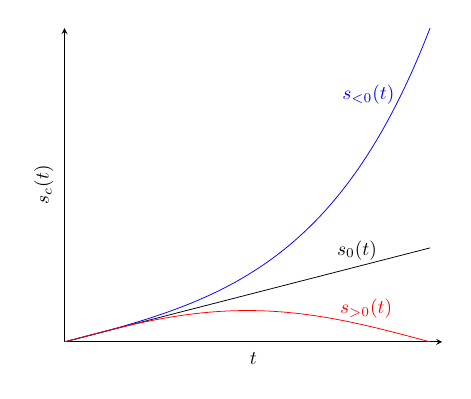
\begin{tikzpicture}[scale=.7]
        \begin{axis}[
            xlabel=$t$,
            ylabel=$s_c(t)$,
            samples=200,
            axis x line=bottom,
            axis y line=left,
            xtick=\empty,
            ytick=\empty,
            xlabel near ticks,
            ylabel near ticks,
            xmin=0, xmax=3.1,
        ]
            \addplot[domain=0:3] {x}
                node[pos=0.8, above] {$s_0(t)$};
            \addplot[domain=0:3, blue] {sinh(x)}
                node[pos=0.8, left, blue] {$s_{<0}(t)$};
            \addplot[domain=0:3, red] {sin(180 / 3 *x)}
                node[pos=0.8, above, red]{$s_{>0}(t)$};
        \end{axis}
    \end{tikzpicture}
\end{marginfigure}
Given $c \in \mathbb{R}$, consider the following function \[
s_c: \mathbb{R} \to \mathbb{R}
\] defined as 
\begin{equation}
    \label{eq:curvfunc}
    s_c(t):=
    \begin{cases}
        \frac{1}{\sqrt{c}}\sin(\sqrt{c}t) & c > 0\\
        t &c=0\\
        \frac{1}{\sqrt{-c}} \sinh(\sqrt{-c}t) &c<0 
    \end{cases}
\end{equation}
\begin{eg}
    Let us consider several model manifolds for constant sectional curvature.
    \begin{enumerate}
        \item The $n$-dimensional Euclidean space $(\mathbb{R}^n, g_\text{st})$ with the Euclidean metric and the $n$-dimensional Minkowski space $(\mathbb{R}^{1,n-1}, \eta)$ with the Minkowski metric have $c \equiv 0$. In polar coordinates, we have \[
                g_\text{st}=dr^2 + r^2 \mathring{g}_{n-1}=dr^2 + s_{0}(r)^2 \mathring{g}_{n-1}
        \] and \[
        \eta = -d\tau^2 + \tau^2 \hcirc{g}=-d\tau^2 + s_0(\tau)^2 \hcirc{g}_{n-1}
        .\] 
    \item The $n$-sphere $(\mathbb{S}^n, \mathring{g}_n)$ with the round metric has $c \equiv 1$. In polar coordinates, we have \[
            \mathring{g}_n=d\theta^2 + \sin^2(\theta) d\phi^2 = d\theta^2+s_1(\theta)^2d\phi^2
    .\]  
\item The hyperbolic $n$-space $(\mathbb{H}^n, \hcirc{g}_n)$ with the hyperbolic metric has $c \equiv -1$. In polar coordinates, we get \[
        \hcirc{g}_n= d\xi^2 + \sinh(\xi)^2 \mathring{g}_{n-1}=d\xi^2+s_{-1}(\xi)^2 \mathring{g}_{n-1}
.\] 
    \end{enumerate}
\end{eg}
\begin{prop}[Jacobi Fields in Constant Curvature Spaces]
    \label{prop:jacobiinconst}
    Let $(M,g)$ be a SRMF with constant sectional curvature $c \in \mathbb{R}$ and let $\gamma: I \to \mathbb{R}$ be a unit-speed geodesic with $0 \in I$. Then some $J \in \mathfrak{X}(\gamma)^\perp$ with $J(0)=0$ and $\nabla_{\frac{\d}{\d t}} J(0) \neq 0$ satisfies $J \in \mathfrak{J}(\gamma)$ if and only if
    \begin{equation}
        \label{eq:jacobiconcur}
        J(t)=k \cdot s_{\epsilon c}(t) \cdot E(t)
    \end{equation} for some $k \in \mathbb{R}$, $\epsilon := \langle \dot{\gamma},\dot{\gamma}  \rangle$ and parallel $E \in \mathfrak{X}(\gamma)^\perp$ with $\|E\|^2=1$.   
\end{prop}

\begin{proof}
$(\Leftarrow)$: We do one auxilliary computation beforehand: The second derivative of $s_\alpha (t)$ for some parameter $\alpha \in \mathbb{R}$ is:
\[
    \ddot{s}_\alpha (t)=
    \begin{cases}
        \frac{d}{dt} \cos(\sqrt{\alpha}t) = - \sqrt{\alpha} \sin(\sqrt{\alpha}t)&\alpha > 0\\
        \frac{d}{dt} 1 =0&\alpha = 0\\
        \frac{d}{dt} \cosh(\sqrt{-\alpha}t)=\sqrt{-\alpha} \sinh(\sqrt{-\alpha}t) &\alpha<0
    \end{cases} = - \alpha s_\alpha (t).\]\marginnote{Note that in the $\alpha < 0$-case, we multiply with negative $\alpha$ in the end, so the sign switch is intentional and correct.}
    Directly calculating the Jacobi equation yields:
    \begin{align*}
        \nabla_{\frac{d}{dt}}^2 J(t)-R(J,\dot{\gamma})\dot{\gamma}&= \nabla_{\frac{d}{dt}}^2 (k s_{\epsilon c}(t)E(t))+ks_{\epsilon c}(t)R(E,\dot{\gamma})\dot{\gamma}\\
                                                                  &\eqnmark[blue]{node4}{=} k \ddot{s}_{\epsilon c}(t)E(t) + ks_{\epsilon c}(t)\nabla_{\frac{d}{dt}}(\cancel{\nabla_{\frac{d}{dt}} E(t)}) \\
                                                                  & \, \, + ks_{\epsilon c} c(\|\dot{\gamma}\|^2 E(t)- \cancel{\langle E,\dot{\gamma}  \rangle} \dot{\gamma} ) \\
                                                                  &=-kc\epsilon s_{\epsilon c}(t)E(t)+kc\epsilon s_{\epsilon c}(t)E(t)=0,
    \end{align*}
    \annotate[yshift=0.6em]{below, left}{node4}{Lemma \ref{lem:concurveq}}
    where we used that $E$ is parallel and normal and $\gamma$ is unit-speed.
    $(\Leftarrow):$ The goal is to find $k$ and $E$ such that $J(0)=J_{k,E}(0)$ and $\nabla_{\frac{d}{dt}}J(0)=\nabla_{\frac{d}{dt}}J_{k,E}(0)$. Then we can apply uniqueness of Jacobi fields to obtain the claim.
    \begin{enumerate}
        \item $J(0)=J_{k,E}$ holds by assumption.
        \item We have \[
                \nabla_{\frac{d}{dt}}J(0)=k\dot{s}_{\epsilon c}(0)E(0)=kE(0) 
            .\] 
            This agrees with our vector field if we choose $k:=\|\nabla_{\frac{d}{dt}} J(0)\|$ and $E(0):=\frac{1}{k}\nabla_{\frac{d}{dt}}J(0)$ which is well-defined since $k \neq 0$ by assumption. We extend this by using the parallel transport 
            $P_{\gamma(t)}$ along $\gamma$ to define $E(t):=P_{\gamma(t)}E(0)$. We have already seen that \[
                E(t) \perp \dot{\gamma}(t) \iff E(0) \perp \dot{\gamma}(0) \iff \nabla_{\frac{d}{dt}}J(0) \perp \dot{\gamma}(0) 
            ,\] and the last statement is part of our assumption.
    \end{enumerate}
\end{proof}
\begin{remark}
    \begin{enumerate}
        \item If $(M,g)$ is Riemannian (or Lorentzian and $\gamma$ timelike), $J \in \mathfrak{J}(\gamma)^\perp$ already implies $\nabla_{\frac{d}{dt}}J(0)\perp \dot{\gamma}(0)$ and $\dot{\gamma}(0)^\perp \subseteq T_{\gamma(0)}M$ spacelike, so $\nabla_{\frac{d}{dt}}J(0)\neq 0$.  
        \item In constant curvature spaces, we have now two forms for Jacobi fields, $J(t)=tw^i\partial_i|_{\gamma(t)}$ and $J(t)=ks_{\epsilon c}(t)E(t)$.
    \end{enumerate}
\end{remark}
Our goal is now to obtain the first general result with help of Jacobi fields.
We will need the notion of a radial distance function and the associated vector field.
\marginnote{
    Given a time-oriented Lorentzian manifold, we define the radial distance function by the proper time $\tau: I^U(p) \to \mathbb{R}$ with $\tau(q):=\tau_U(p,q)>0$. This yields a field $\partial_\tau$.
}
Given a Riemannian manifold $(M,g)$ and a normal chart $(U, x^i)$ around some $p \in M$. Define the \textbf{radial distance function} $r: U \to \mathbb{R}$ by $r(q)=d(p,q) >0$. If the coodinates are centered at $p$, we have the explicit form \[
    r(x)=\sqrt{(x^1)^2 + \cdots + (x^n)^2}
,\] and on $U \setminus \{p\}$ we get the \textbf{radial vector field} \[
\partial_r = \frac{x^i}{r(x)} \partial_i
.\]  This is smooth on $U \setminus \{p\}$ and independent of choice of charts.
\begin{definition}[Polar Coordinates]
    In the following, $\mathring{g}$ is the round metric and $\hcirc{g}$ is the hyperbolic metric.
    \begin{enumerate}
        \item \textbf{Riemannian polar coordinates} are given by the map
        \begin{align*}
            \Phi_R: (\mathbb{R}_+ \times \mathbb{S}^{n-1}, dr^2+r^2 \mathring{g}_{n-1}) &\to (\mathbb{R}^n \setminus \{0\}, g_\text{st})\\
            (r,\theta)&\mapsto r \iota_{\mathbb{S}^{n-1}}(\theta),
        \end{align*}
        where $\iota: \mathbb{S}^{n-1} \hookrightarrow (\mathbb{R}^n, g_\text{st})$ is any isometric embedding with $\im \iota_{\mathbb{S}^{n-1}}=\left\{x \in \mathbb{R}^n \mid \|x\|=1\right\}$.
    \item \textbf{Lorentian polar coordinates} are the map
        \begin{align*}
            \Phi_L: (\mathbb{R}_+ \times \mathbb{H}^{n-1}, -d\tau^2+\tau^2 \hcirc{g}_{n-1}) &\to (I^+(0), \eta)\\
            (\tau, \xi)&\mapsto \tau \iota_{\mathbb{H}^{n-1}}(\xi),
        \end{align*}
        where $\iota: \mathbb{H}^{n-1} \hookrightarrow (\mathbb{R}^{1,n-1}, \eta)$ is any isometric embedding with $\im \iota_{\mathbb{H}^{n-1}}=\left\{x \in \mathbb{R}^{1,n-1} \mid \eta(x,x)=-1\right\}$.
    \end{enumerate}
\end{definition}
\begin{theorem}[Constant-Curvature Metrics in Normal Coordinates]
    \label{thm:constcurvmet}
Let $(M,g)$ be a RMF or a \red{LMF} with constant curvature $c \in \mathbb{R}$. Let $U$ be a normal neighbourhood of $p \in M$ and $\psi=(x^i)$ be normal coordinates such that $\psi_\ast g_p=g_\text{st}$. Let $r(q)=\|\exp_p^{-1}(q)\|$ resp. \red{$\tau(q)=\|\exp_p^{-1}(q)\|$} be the radial distance function. Define angle functions $\theta(q):=\iota^{-1}_\mathbb{S} \left(\frac{\exp_p^{-1}(q)}{r(q)}\right)$ and $\red{ \xi(q) := \iota^{-1}_\mathbb{H} \left(\frac{\exp_p^{-1}(q)}{\tau(q)}\right)}$. Then we have isometries 
    \begin{align*}
        \phi:=\Psi_R^{-1}\circ \psi: U \setminus \{p\} &\to \mathbb{R}_+ \times \mathbb{S}^{n-1}\\
        q &\mapsto (r(q),\theta(q))\\
    \red{\phi_L:=\Phi^{-1}_L \circ \psi: I_U^+(p)} \, &\red{\to \mathbb{R}_+ \times \mathbb{H}^{n-1}}\\
        \red{q} \, &\red{\mapsto (\tau(q),\xi(q))}
    \end{align*}
    onto their image between $g$ and \[
        g^c = dr^2 + s_c(r)^2 \mathring{g}_{n-1}
    \] or \[
    \red{g^c = -d\tau^2 + s_c(\tau)^2 \hcirc{g}_{n-1}}
    ,\] respectively.
\end{theorem}
\begin{proof}
    Our goal is to show that for all $q \in U \setminus \{p\}$ and all $w_1,w_2 \in T_{\phi(q)}(\mathbb{R}_+ \times \mathbb{S}^{n-1})$, \[
        g_q(\phi^\ast (w_1),\phi^\ast (w_2))=g^c_{\phi(q)}(w_1,w_2)
        \] holds. We show this only for $w_1=w_2=:w$, since the general case follows by polarization. In the following, denote the Euclidean metric by $\langle \cdot,\cdot  \rangle$. We split \[
\marginnote{$\red{    T_{\phi(q)}(\mathbb{R}_+ \times \mathbb{H}^{n-1}) \cong \spn \{\partial_\tau|_{\tau(q)}\} \oplus T_{\xi(q)}\mathbb{H}^{n-1}
}$}
    T_{\phi(q)}(\mathbb{R}_+ \times \mathbb{S}^{n-1}) \cong \spn \{\partial_r|_{r(q)}\} \oplus T_{\theta(q)}\mathbb{S}^{n-1}
    \] and prove the claim in three parts:
    \begin{enumerate}
        \item  $\marginnote{$\red{g_q(\phi^\ast(\partial_\tau|_{\tau(q)}), \phi^\ast(\partial_\tau|_{\tau(q)})) =-1}$} g_q(\phi^\ast(\partial_r|_{r(q)}), \phi^\ast(\partial_r|_{r(q)})) = g_{\phi(q)}^c (\partial_r|_{r(q)}, \partial_r|_{r(q)}) =1$
        \item $\forall w \in T_{\theta(q)}\mathbb{S}^{n-1}: g_q(\phi^\ast(\partial_r|_{\phi(r)}), \phi^\ast(w))=0$
        \item $
            \forall w \in T_{\theta(q)}\mathbb{S}^{n-1}: g_q(\phi^\ast(w),\phi^\ast(w))=g_{\phi(q)}^c (q)(w,w)=s_c(r(q))^2 \mathring{g}_{n-1}|_{\theta(q)}(w,w) $
\marginnote{\red{$g_q(\phi^\ast(w),\phi^\ast(w))=s_{-c}(\tau(q))^2 \hcirc{g}_{n-1}|_{\xi(q)}(w,w)$}}
    \end{enumerate}
    For 1 and 2, note that \[
        (\Phi_R)_{\ast, (r(q),\theta(q))}(\partial_r)=(\Phi_R^{-1})^\ast(\partial_r|_{\phi(q)}) = \iota(\theta(q)) \in T_{\psi(q)}\mathbb{R}^n
    .\] Since $\psi(q)=r(q)\iota(\theta(q))$, this is radial, hence the Gauß lemma applies. Defining $v:=(\Phi_R^{-1})^\ast(w)$, we get:
    \begin{align*}
        g_q(\phi^\ast(\partial_r|_{\phi(q)}), \phi^\ast(w))&=g_q((\exp_p)_{\ast, \psi(q)} (\iota(\theta(q))), (\exp_p)_{\ast, \psi(q)}(v))\\
                                                           &=g_p(\iota(\theta(q)),v)=\langle \iota(\theta(q)),v  \rangle \\
                                                           &=
                                                           \begin{cases}
                                                               1 &v=\iota(\theta(q)) \iff w = \partial_r|_{\phi(q)}\\
                                                               0 &v \perp \iota(\theta(q)) \eqnmark[blue]{node2}{\iff} w \in T_{\theta(q)}\mathbb{S}^{n-1}
                                                           \end{cases}.
    \end{align*}
    \annotate[yshift=-1em]{below, label below}{node2}{$\Phi_R$ is isometry $g^c \leftrightarrow \langle \cdot,\cdot  \rangle$ }
    This proves 1 and 2 simultaneously.
    \marginnote{Note that we have not used our constant curvature assumption so far. This will become important in chapter \ref{chap:comparision}.}\newline
    Now we turn our attention to 3.: Let $w \in T_{\theta(q)}\mathbb{S}^{n-1}$ and set $v:=(\Phi_R^{-1})^\ast (w) \in T_{\psi(q)}\mathbb{R}^n$.
    We have by definition \[
        g^c_{\phi(q)}(w,w)=s_c(r(q))^2 \mathring{g}_{n-1}|_{\theta(q)}(w,w)=\frac{s_c(r(q))^2}{r(q)^2}\langle v, v \rangle 
    .\]

    \marginnote{\red{This largely goes through for the Lorentzian case, just switch $\Phi_R$ for $\Phi_L$ and use $s_{-c}(t)$. Note that $J$ is normal to a timelike geodesic, so the sign is still positive.}}
    Let $J$ be the unique Jacobi field along the unit-speed radial geodesic $\gamma: [0,b] \to U$ from $p$ to $q$ ($b=r(q)$) with $J(0)=0$ and $J(b)=\phi^\ast(w) \in T_qM$. We have $\dot{\gamma}(b) \propto \phi^\ast_{r(q),\theta(q)}(\partial_r)\perp \phi^\ast(w)$, so $J \in \mathfrak{J}(\gamma)^\perp$. This means we can write \[
    J(t)=ks_c(t)E(t)
    \] with $E(b) \propto \phi^\ast(w)$. We calculate explicitly:
    \[
        k^2 = g_p(\nabla_{\frac{d}{dt}}J(0), \nabla_{\frac{d}{dt}}J(0))
    \]
    and obtain \[
        \|\phi^\ast(w)\|^2_{g_q} = \|J(b)\|^2_{g_q} = k^2 s_c(b)^2=s_c(r(q))^2 \|\nabla_{\frac{d}{dt}}J\|^2_{g_p}
    .\] Now rescale $\gamma$ to $[0,1] \to M$ and use $\phi^\ast(w)=\psi^\ast(v)=v^i\partial_i|_q \in T_qM$ to get $J(t)=\frac{t}{b}v^i\partial_i|_{\gamma(t)}$. With this, we calculate \[
    \|\nabla_{\frac{d}{dt}}J(0) \|^2_{g_p} = \|\frac{1}{b}v^i\partial_i|_{\gamma(0)}\|^2_{g_p}=\frac{1}{b^2}\langle v,v  \rangle 
    \] With this, claim 3 follows.
\end{proof}
\begin{corollary}
    \marginnote{\red{The Lorentzian case is a bit harder to phrase, but the idea still holds. The problem is that families of Riemannian metrics on $\mathbb{H}^{n-1}$ are generally not globally definable on $\mathbb{H}^{n-1}$ as $\psi(I_U^+(p))$ does not contain an entire $\mathbb{H}^{n-1}_\tau$, no matter how small $\tau$ is.}}
    Let $(M,g)$ be a RMF, $p \in M$ and $U$ a normal neighbourhood with normal coodinates $\psi$ such that $\psi_\ast g_p = g_\text{st}$. Let $\epsilon >0$ such that $B_\epsilon(0) \subseteq \psi(U)$. Then we find a family $\left\{h(r) \mid r \in (0, \epsilon)\right\}$ of Riemannian metrics on $\mathbb{S}^{n-1}$ such that \[
        \phi: \Phi_R^{-1} \circ \psi: B_\epsilon^{d_g}(p)\setminus \{p\} \to (0,\epsilon) \times \mathbb{S}^{n-1}
    \] given again by $\phi(q):=(r(q),\theta(q))$ is a bijective isometry between $g$ and $dr^2+h(r)$.
\end{corollary}
\begin{proof}
    We know that $B_\epsilon^{d_g}(p)=\psi^{-1}(B_\epsilon(0))$ by theorem \ref{thm:metrizationriem}. Let $r \in (0,\epsilon)$, $\theta \in \mathbb{S}^{n-1}$ and $w_1,w_2 \in T_\theta \mathbb{S}^{n-1}$. We define \[
        h(r)(w_1,w_2):=g_{\phi^{-1}(r,\theta)}(\phi^{-1}_{\ast, (r,\theta)}(0 \partial_r+w_1), \phi^{-1}_{\ast,(r,\theta)}(0 \partial_r + w_2))
    .\] This is a smooth, symmetric, non-degenerate $(0,2)$-tensor field on $\mathbb{S}^{n-1}$. $\phi$ being an isometry follows from the definition of $h(r)$, 1, and 2 of the previous proof.
    
\end{proof}
\begin{corollary}[Constant Curvature implies local Isometry]
   All Riemannian and Lorentzian manifolds of constant curvature are locally isometric. 
\end{corollary}
\begin{proof}
    \marginnote{The Riemannian case is easier and can be found in \cite{LeeRM}. The theorem also holds for the semi-Riemannian case in general with a different proof, found in \cite{ONeill10}.}
    We do the Lorentzian case. Given LMFs $(M_1,g_1)$ and $(M_2,g_2)$ with $p_i \in M_i$, we want to show that there are open neighbourhoods $U_i \subseteq M_i$ and a local isometry $\phi: (U_1,g_1) \overset{\cong}\to (U_2,g_2)$. So let $\widetilde{U}_i$ be convex neighbourhoods of $p_i$, $p_i^- \ll_{\widetilde{U}_i} p_i$ and $\tau_{\widetilde{U}_1}(p_1^-,p_1)=\tau_{\widetilde{U}_2}(p_2^-,p_2)=\epsilon$. Choose normal coordinates at $p_i^-$ such that $\psi_i(p_i)=(\epsilon,0,\dots,0)$. Consider polar-normal coordinates \[
        \phi_i: \widetilde{U}_i \to V_i \subseteq (0,\infty) \times \mathbb{H}^{n-1}
    .\] They satisfy \[
    \phi_1(p_1)=\phi_2(p_2)=:(\epsilon, \xi_0) \in V_1 \cap V_2,
\] so $V_1 \cap V_2$ is an open neighbourhood of $(\epsilon, \xi_0)$. Setting $U_i := \phi_i^{-1}(V_1 \cap V_2)$, we obtain the desired isometry \[
\phi := \phi_2^{-1} \circ \phi_1: U_1 \overset{\cong}\to U_2
.\]  
\end{proof}
\section{Conjugate Points}
\label{sec:conjpoints}

\begin{definition}[Regular and Critical Points]
    Let $M,N$ be smooth manifolds and $F: M \to N$ be a smooth map. We call $p \in M$ a \textbf{regular point} of $F$ if $F_{\ast, p}:T_pM \to T_{F(p)}N$ is surjective. Otherwise, we call $p$ a \textbf{critical point}. We denote the critical points by $\crit F$.
\end{definition}

Consider the exponential map $$\exp_p: T_pM \to M$$. The inverse function theorem guarantees that locally around all regular points, $\exp_p$ is a diffeomorphism. What happens at critical points?
\begin{ex}
    Consider $\mathbb{S}^2$. Given the unit circle $S_0 := \left\{v \in T_p\mathbb{S}^2 \mid \|v\|=\pi \right\} \subseteq T_p\mathbb{S}^2$, the image, which is the antipodal point to $p$, consists only of critial points of $\exp_p$. At that point, several things happen:
    \begin{enumerate}
        \item Jacobi fields admit zeros: Given $J(t)=k s_1(t)E(t)=k\sin(t)E(t)$, we have $J(0)=J(\pi)=0$.
        \item All unit-speed geodesics originating at $p$ meet at the antipodal point at $t=\pi$.
        \item All these geodesics stop being minimizing after $t=\pi$.
    \end{enumerate}
    The question is, which of these hold generally?
\end{ex}
\begin{definition}[Conjugate Points]
    Let $(M,g)$ be a SRMF, $\gamma:I \to M$ be a geodesic, $a,b \in I$, and $\gamma(a):=p$, $\gamma(b):=q$. We call $p$ \textbf{conjugate} to $q$ along $\gamma$ if there exists a non-zero Jacobi field $J \in \mathfrak{J}(\gamma)$ with $J(a)=J(b)=0$. We call the dimension of the subspace of Jacobi fields vanishing at $a$ and $b$ the \textbf{order} or \textbf{multiplicity} of conjugacy.
\end{definition}
\begin{remark}
    Let $\gamma$ be a timelike or spacelike geodesic. If there is a Jacobi field witnessing conjugacy, we can always choose a normal one satisfying the same condition since \[
        J^\top = (kt+d)\dot{\gamma}(t)
    ,\] which vanishes at most at one point. Hence the order of conjugacy is always $\leq \dim M -1$.
\end{remark}
\begin{prop}[Conjugacy and Critical Points]
    Let $(M,g)$ be a SRMF, $p \in M$, $v \in \mathcal{E}_p$, and let $\gamma=\gamma_v: [0,1] \to M$ be the unique geodesic with $\gamma(0)=p$ and $\dot{\gamma}(0)=v$. Set $q := \gamma_v(1)=\exp_p(v)$.
    Then $p$ is conjugate to $q$ along $\gamma$ if and only if $v \in \crit(\exp_p)$.
\end{prop}
\begin{proof}
    $(\Leftarrow):$ Let $v \in \crit(\exp_p)$. We find $w \in T_pM$ such that $(\exp_p)_{\ast, v}(w)=0$ but $w \neq 0$. Take a Jacobi field with initial data $J(0)=0$ and $\nabla_{\frac{d}{dt}}J(0)=w$. By lemma \ref{lem:jacobigeodvar}, we can write $J$ as variation field of the geodesic variation \[
        \Gamma (s,t):=\exp_p (t(v+sw))
    .\] We have \[
    J(1) = \left. \frac{\partial}{\partial s}\right|_{s=0} \Gamma(s,1)= \left. \frac{\partial}{\partial s}\right|_{s=0} \exp_p(v+sw)=(\exp_p)_{\ast, v}(w)=0
    .\] 
$(\Rightarrow):$ Let $J$ be a non-zero Jacobi field along $\gamma$ with $J(0)=J(1)=0$. Writing $w:=\nabla_{\frac{d}{dt}}J(0) \neq 0$ and again $J$ as variation field of \[
\Gamma (s,t)=\exp_p(t(v+uw))
\] yields $J(1)=0=(\exp_p)_{\ast,v}(w)$, so $(\exp_p)_{\ast, v}$ fails to be injective.  
\end{proof}
If $(M,g)$ is a SRMF and $\gamma: I \to M$ is a geodesic, the \textbf{two-point boundary value problem} asks whether it is always possible to find a Jacobi field along $\gamma$ with two prescribed boundary values $J(0)=v \in T_{\gamma(0)}M$ and $J(1)=w \in T_{\gamma(1)}M$.
\begin{prop}[The two-point Boundary Value Problem]
    Let $(M,g)$ be a SRMF and $\gamma: [a,b] \to M$ be a geodesic segment. The two-point boundary value problem is solvable if and only if $\gamma(a)$ is not conjugate to $\gamma(b)$.
\end{prop}
\begin{ex}
    Prove the preceeding proposition.
\end{ex}
\begin{prop}[Conjugacy and Sectional Curvature]
    Let $(M,g)$ be a RMF with non-positive sectional curvature. For any $p \in M$ and any geodesic $\gamma: [0,b] \to M$ originating at $p$, there are no points conjugate to $p$ along $\gamma$.
\end{prop}
\begin{ex}
    Prove the preceeding proposition.
\end{ex}
\section{The Second Variation Formula for Arc-Length}
\label{sec:secondvar}
\begin{theorem}[Second Variation Formula for Arc-Length]
    Let $(M,\langle \cdot,\cdot  \rangle )$ be a SRMF, $\gamma: [a,b]\to M$ be a unit-speed geodesic segment, and let \[
        \Gamma: (-\delta, \delta) \times [a,b] \to M
    \] be a continuous, fixed-endpoint variation of $\gamma$ such that all curves $t \mapsto \Gamma_s(t)$ have the same causal character. Additionally, let there be a partition $\{t_i\}_{1\leq i \leq n}$ of $[a,b]$ such that $\Gamma|_{[t_i,t_{i+1}]}$ is smooth with $t_1=a$ and $t_n=b$.
    Then the \textbf{second variation of arc-length} is given by 
    \begin{equation}
        \label{eq:secvar}
        \marginnote{Note that the sign change in \cite{LeeRM} originates from switching the second and third entry of the Riemann tensor.}
        \left.\frac{d^2}{ds^2}\right|_{s=0}L[\Gamma_s] = \epsilon \int_a^b \left(\Rm(V^\perp, \dot{\gamma}, V^\perp, \dot{\gamma})+\langle \nabla_{\frac{d}{d t}} V^\perp, \nabla_{\frac{d}{d t}}V^\perp  \rangle \right)dt
    \end{equation}
    where $\epsilon = \langle \dot{\gamma},\dot{\gamma}  \rangle$, $V= \left. \frac{\partial}{\partial s}\right|_{s=0} \Gamma$, and $V^\perp = V - \epsilon \langle \dot{\gamma}, \dot{\gamma} \rangle \dot{\gamma}$.
\end{theorem}
\begin{proof}
    The proof is done by direct calculation. We set $\left. \frac{\partial}{\partial s}\right|_{s=0} \Gamma =:S(s,t)$ and $\left. \frac{\partial}{\partial t}\right|_{t=0} \Gamma := T(s,t)$. We have 
            \begin{align*}
                \frac{d^2}{ds^2} L[\Gamma_s]&=\frac{d}{ds} \int_{t_i}^{t_{i+1}} \frac{\partial}{\partial s} \langle \dot{\Gamma}_s,\dot{\Gamma}_s  \rangle dt =   \frac{d}{ds} \int_{t_i}^{t_{i+1}} \frac{\epsilon \langle \nabla_{\frac{d}{d s}}  T, T  \rangle }{\sqrt{\epsilon \langle T,T  \rangle }}dt\\
                                            &= \epsilon \int_{t_i}^{t_{i+1}} \frac{\partial}{\partial s} \frac{\langle \nabla_{\frac{d}{d s}} S, T \rangle}{\sqrt{\epsilon \langle T,T  \rangle }} dt \\
                                            &= \epsilon \int_{t_i}^{t_{i+1}} \left[ \frac{\langle \nabla_{\frac{d}{d s}} \nabla_{\frac{d}{d t}} S,T  \rangle + \langle \nabla_{\frac{d}{d t}} S, \nabla_{\frac{d}{d s}} T  \rangle  }{\sqrt{\epsilon \langle T,T  \rangle }} - \frac{\langle \nabla_{\frac{d}{d t}} S,T  \rangle \langle \nabla_{\frac{d}{d s}} T,T  \rangle  }{(\epsilon \langle T,T  \rangle )^{\frac{3}{2}}} \right] dt \\
                                            &= \epsilon \int_{t_i}^{t_{i+1}} \left[ \frac{\langle \nabla_{\frac{d}{d s}} \nabla_{\frac{d}{d t}} S,T  \rangle + \langle \nabla_{\frac{d}{d t}} S, \nabla_{\frac{d}{d t}} S  \rangle  }{\sqrt{\epsilon \langle T,T  \rangle }} - \frac{\langle \nabla_{\frac{d}{d t}} S,T  \rangle \langle \nabla_{\frac{d}{d t}} S,T  \rangle  }{(\epsilon \langle T,T  \rangle )^{\frac{3}{2}}} \right] dt 
            \end{align*}

            Evaluating at $s=0$ yields $\frac{\partial}{\partial t} \Gamma(0,t)=\dot{\gamma}(t)$ and hence $\langle T ,T  \rangle = \epsilon$. Also, we obtain $\nabla_{\frac{d}{d s}} S (0,t)=\nabla_{\frac{d}{d t}} V$. This yields 
            \[
                \left. \frac{d^2}{ds^2}\right|_{s=0} L[\Gamma_s] = \epsilon \int_{t_i}^{t_{i+1}} \left[ \underbrace{\langle \nabla_{\frac{d}{d s}} \nabla_{\frac{d}{d t}} S,\dot{\gamma}  \rangle}_{=:A}  + \underbrace{\langle \nabla_{\frac{d}{d t}} V, \nabla_{\frac{d}{d t}} V \rangle}_{=:B} - \underbrace{\epsilon \langle \nabla_{\frac{d}{d t}} V, \dot{\gamma}  \rangle^2}_{=:C}  \right] dt
            .\] 
            Term $A$ can be simplified by lemma \ref{lem:curvlem} to:
            \begin{align*}
                A|_{s=0} &= \langle \nabla_{\frac{d}{d t}} \nabla_{\frac{d}{d s}} S (0,t),\dot{\gamma}  \rangle + \langle \R(S(0,t),T(0,t))S(0,t), \dot{\gamma} \rangle\\ 
                         &= \langle \nabla_{\frac{d}{d t}} \nabla_{\frac{d}{d s}}  S(0,t),\dot{\gamma}  \rangle + \langle R(V,\dot{\gamma})V,  \dot{\gamma}\rangle   \\
                         \marginnote{That the only contribution is from the normal part follows either by direct calculation or by using the symmetry $Rm(\cdot, \cdot, v, v)=\Rm(v,v,\cdot,\cdot)=0$.}
                         &= \Rm(V^\perp, \dot{\gamma}, V^\perp, \dot{\gamma})+\langle \nabla_{\frac{d}{d t}} \nabla_{\frac{d}{d s}} S(0,t),\dot{\gamma}  \rangle 
            \end{align*}
            Term $B$ can be written as \[
                \langle \nabla_{\frac{d}{d t}} V,\nabla_{\frac{d}{d t}} V  \rangle = \langle (\nabla_{\frac{d}{d t}} V)^\perp, (\nabla_{\frac{d}{d t}} V)^\perp  \rangle + \langle \nabla_{\frac{d}{d t}} V, \dot{\gamma} \rangle ^2 \epsilon
            .\] A direct calculation shows that taking the normal part commutes with the covariant derivative: \[
            \marginnote{All other Leibniz rule terms vanish since $\gamma$ is a geodesic segment.}
            \nabla_{\frac{d}{d t}} V^\perp = \nabla_{\frac{d}{d t}}V-\epsilon \nabla_{\frac{d}{d t}} \langle V,\dot{\gamma}  \rangle \dot{\gamma} = \nabla_{\frac{d}{d t}} V - \epsilon \langle \nabla_{\frac{d}{d t}} V, \dot{\gamma} \rangle \dot{\gamma} = (\nabla_{\frac{d}{d t}} V)^\perp 
            .\] This yields \[
            \langle \nabla_{\frac{d}{d t}} V, \nabla_{\frac{d}{d t}} V \rangle = \langle \nabla_{\frac{d}{d t}} V^\perp, \nabla_{\frac{d}{d t}} V^\perp \rangle + \langle \nabla_{\frac{d}{d t}} V, \dot{\gamma} \rangle^2   
            .\] However, the rightmost term cancels with $C$. 
            It remains to show that \[
                \epsilon \int_{t_i}^{t_{i+1}} \langle \nabla_{\frac{d}{d t}} \nabla_{\frac{d}{d s}} S(0,t),\dot{\gamma}  \rangle dt 
            \] vanishes when summing over $i$.
We have: 
\begin{align*}
    \sum_{i=1}^n\int_{t_i}^{t_{i+1}} \langle \nabla_{\frac{d}{d t}} \nabla_{\frac{d}{d s}} S(0,t),\dot{\gamma}  \rangle dt &= \sum_{i=1}^n\int_{t_i}^{t_{i+1}} \frac{d}{dt} \langle \nabla_{\frac{d}{d s}} S(0,t),\dot{\gamma}  \rangle dt \\
                                                                                                                           &=  \sum_{i=1}^n \left( \langle \nabla_{\frac{d}{d s}} S(0,t_{i+1}),\dot{\gamma}(t_{i+1})  \rangle - \langle \nabla_{\frac{d}{d s}} S(0,t_i),\dot{\gamma}(t_i)  \rangle  \right)\\  
                                                                                                                           &= \langle \nabla_{\frac{d}{d s}} S(0,b), \dot{\gamma}(b)  \rangle - \langle \nabla_{\frac{d}{d s}} S(0,s),\dot{\gamma}(a)  \rangle = 0 ,
\end{align*} 
where we used that $\Gamma$ is a variation with fixed endpoints in the last step.
\end{proof}
There is also a slightly different version:
\begin{prop}[Second Variation for Submanifolds]
    \label{prop:secvarumf}
    Let $(M,g)$ be a RMF or LMF and $\Sigma_1,\Sigma_2$ be two \red{spacelike} submanifolds. Let $\gamma: [a,b]\to M$ be a \red{timelike} unit-speed geodesic segment meeting $\Sigma_1$ orthogonally at $t=a$ and $\Sigma_2$ orthogonally at $t=b$. Let $\Gamma$ be a continuous variation of $\gamma$ which is smooth on some partition of $[a,b]$, and with $\Gamma(s,a) \in \Sigma_1$ and $\Gamma(s,b)\in \Sigma_2$ for all $s$. Let $\sff_i$ be the second fundamental form of $\Sigma_i$, and let $\epsilon = \langle \dot{\gamma}, \dot{\gamma} \rangle$. Then the second variation of arc-length is given by
    \begin{align*}
        \epsilon \left.\frac{d^2}{ds^2}\right|_{s=0} L[\Gamma_s] = \int_a^b &\left[ \langle \nabla_{\frac{d}{d t}} V^\perp,\nabla_{\frac{d}{d t}} V^\perp  \rangle + \Rm(V^\perp, \dot{\gamma}, V^\perp, \dot{\gamma}) \right] dt \\
                                                                   &+ \langle \sff_2(V(b),V(b)),\dot{\gamma}(b)  \rangle - \langle \sff_1(V(a),V(a)),\dot{\gamma}(a)  \rangle 
    \end{align*}
\end{prop}
\begin{ex}
    Prove the preceeding proposition.
\end{ex}
The second variation behaves a bit like the Hessian in real analysis on $\mathbb{R}^n$: It tells us something about the maxima and minima of the length functional. We use this to define something akin to a Hessian for vector fields.
\begin{notation}
    We denote the space of piecewise smooth vector fields along a curve $\gamma$ by $\overline{\mathfrak{X}}$. If $\gamma: [a,b] \to M$, we denote the space of vector fields with $X(a)=X(b)=0$ by $\mathfrak{X}_0$.
\end{notation}
\begin{definition}[Index Form]
    Let $(M,\langle \cdot,\cdot  \rangle )$ be a SRMF and $\gamma:[a,b] \to M$ be a unit-speed geodesic segment. We define the \textbf{index form} to be a map \[
    I: \overline{\mathfrak{X}}(\gamma)^\perp \times \overline{\mathfrak{X}}(\gamma)^\perp \to \mathbb{R}
    \]  given by \[
    I(X,Y):= \epsilon \int_a^b (\langle \nabla_{\frac{d}{d t}} X,\nabla_{\frac{d}{d t}} Y  \rangle + \Rm(X,\dot{\gamma},Y, \dot{\gamma})) dt 
    .\] 
\end{definition}
\begin{corollary}[Index Form and Extremizing Behaviour]
    \label{cor:indexform}
    \marginnote{\red{
        Let $(\mathcal{L},g)$ be a time-oriented LMF and $\gamma: [a,b] \to \mathcal{L}$ be a unit-speed future-directed timelike geodesic segment. If there exists a non-zero $V \in \overline{\mathfrak{X}}_0(\gamma)^\perp$ such that} \[
        \red{I(V,V)>0
,}\] \red{then $\gamma$ cannot maximize the distance from $\gamma(a)$ to $\gamma(b)$.}}
    Let $(M,g)$ be a RMF and $\gamma: [a,b] \to M$ be a unit-speed geodesic segment. If there exists $V \in \overline{\mathfrak{X}}_0(\gamma)^\perp$ such that \[
    I(V,V)<0
    ,\] then $\gamma$ cannot minimize the distance from $\gamma(a)$ to $\gamma(b)$.
\end{corollary}
\begin{remark}
    \marginnote{\red{In the Lorentzian case, maximizing $\gamma$ implies negative semi-definity.}}
    We can also phrase this as if $\gamma$ is minimizing from $\gamma(a)$ to $\gamma(b)$, then $I|_{  \overline{\mathfrak{X}}_0(\gamma)^\perp \times \overline{\mathfrak{X}}_0(\gamma)^\perp}$ is positive semi-definite.
\end{remark}
\begin{corollary}[Sectional Curvature and Submanifolds]
    Let $(M,g)$ be a connected, complete RMF with positive sectional curvature. If $\Sigma_1, \Sigma_2$ are compact, totally geodesic submanifolds such that \[
    \dim \Sigma_1 + \dim \Sigma_2 \geq \dim M
    ,\] then $\Sigma_1 \cap \Sigma_2 \neq \emptyset$.
\end{corollary}
\begin{ex}
   Prove the preceeding corollary. 
\end{ex}
\section{The Theorems of Bonnet-Myers and Hawking}
\label{sec:bonnmyhaw}
Our goal in this section is to control the diameter of certain Riemannian and Lorentzian manifolds. Given a Riemannian manifold $(M,g)$, we define its \textbf{diameter} by 
\[
    \marginnote{\red{Note that in the Lorentzian case, $d_g=\tau$.}}
    \diam_g(M)=\sup_{p,q \in M} d_g(p,q)
.\] 
\subsection*{The Theorem of Bonnet-Myers}
\label{subsec:bonnmys}
\begin{theorem}[Bonnet-Myers]
    Let $(M,g)$ be a complete Riemannian $n$-manifold such that there exists a constant $c \in \mathbb{R}$ with $\Ric_g \geq c>0$ on all of $M$. Then \[
        \diam_g(M) \leq \pi \sqrt{\frac{n-1}{c}}
    .\] 
\end{theorem}
\begin{proof}
    Let $p,q \in M$ be arbitrary. Since $M$ is complete, there is a unit-speed minimizing geodesic $\gamma: [0,b] \to M$ such that $b=L[\gamma]=d_g(p,q)$. Let $f: [0,b] \to M$ be a smooth function with $f(0)=f(b)=0$. Let $(E_i)_{1\leq i \leq n-1}$ be a parallel ONF for $\dot{\gamma}^\perp$. Define vector fields $V_i(t):=f(t)E_i(t)$ along $\gamma$, so $V_i \in \overline{\mathfrak{X}}_0(\gamma)^\perp$ for all $i$. Since $\gamma$ is minimizing, Corollary \ref{cor:indexform} tells us that the index form has to be positive on $V_i$, yielding:
    \begin{align*}
        I(V_i,V_i)&=\int_0^b \left[ \|\nabla_{\frac{d}{dt}} V_i\|^2 - \Rm(V_i, \dot{\gamma}, \dot{\gamma}, V_i)\right] dt\\
                  &= \int_0^b \left[\|\nabla_{\frac{d}{dt}} (fE_i)\|^2 - \Rm(fE_i,\dot{\gamma},\dot{\gamma}, E_i)\right] dt\\
                  &\eqnmark[blue]{node}{=}\int_0^b \left[\dot{f}^2-f^2 \Rm(E_i,\dot{\gamma},\dot{\gamma},E_i)\right] dt.
    \end{align*}
    \annotate[yshift=.1em]{left, label below}{node}{$E_i$ parallel}
    Now we sum over $1 \leq i \leq n-1$:
\end{proof}
\subsection*{Hawking's Singularity Theorem}

\lecture{Exercise Class 14.01.2026}
\label{subsec:hawking}
\begin{theorem}[Hawking's Singularity Theorem]
    Let $(\mathcal{L},\langle \cdot,\cdot  \rangle )$ be a globally hyperbolic Lorentzian $n$-manifold with $\Ric(X,X)\geq 0$ for all $X \in T_pM^\text{t.l.}$ and $p \in M$. If there exists a spacelike hypersurface $\Sigma$ such that:
    \begin{enumerate}[(a)]
        \item $J_-(\Sigma)\cap J_+(q)$ is compact for all $q \in J_-(\Sigma)$.
        \item There exists $\beta > 0$ such that $\langle H_p,N_p  \rangle \geq \beta >0$ for all $p \in \Sigma$, where $N$ is the past-pointing timelike unit normal vector field to $\Sigma$ and $H_p$ is the mean curvature vector, i.e. $$H_p := \frac{1}{n-1}\tr_\Sigma \sff_p = \frac{1}{n-1} \sum_{i=i}^{n-1} \sff_p(E_i,E_i)$$ for any orthonormal frame $E_i$ of $T_p \mathcal{L}|_\Sigma$.
    \end{enumerate}
    Then \[
    \tau_\Sigma (q) =\sup \left\{\tau(q,x) \mid x \in \Sigma \right\} \leq \frac{1}{\beta}
    .\] 
\end{theorem}
\begin{proof}
      Let $q \in J^-(\Sigma)$. By assumption (a) and strong causality, which follows from global hyperbolicity by a previous exercise, there exists a future-directed timelike unit-speed geodesic $\gamma: [0,b] \to \mathcal{L}$ from $q$ to $\Sigma$ with $\dot{\gamma}(b) \perp T_{\gamma(b)}\Sigma$ and $b=L[\gamma]=\tau_\Sigma(q)$. Let $(E_i)_{1 \leq i \leq n-1}$ be a parallel ONF for $\dot{\gamma}^\perp$ along $\gamma$. Consider vector fields $V_i := fE_i$ for some $f$ with $f(0)=0$ and $f(b)=1$. Let $\Gamma_i$ be a variation of $\gamma$ with variational vector field $V_i$, and such that $\Gamma_i(s,0)=q$ as well as $\Gamma_i(s,b) \in \Sigma$ for all $s$. This is possible since $V_i(0)=0$ and $V_i(b) \in T_{\gamma(b)} \Sigma$. Since $L[\gamma]=\tau_\Sigma(q)$, proposition \ref{prop:secvarumf} yields \[
               0 \geq \left. \frac{d^2}{ds^2}\right|_{s=0} L[\Gamma_{i,s}]
       \] for all $i$. We sum over $i$ to obtain:
       \begin{align*}
           0 &\geq \sum_{i=1}^{n-1} \left.\frac{d^2}{ds^2}\right|_{s=0} L[\Gamma_{i,s}]\\
             &= \epsilon \left[ \int_0^b \dot{f}^2 (n-1) - \sum_{i=1}^{n-1} \Rm(fE_i, \dot{\gamma},\dot{\gamma},fE_i) \right] dt + \sum_{i=1}^{n-1} \langle \sff(E_i,E_i),\dot{\gamma}(b)  \rangle \\
             &=-(n-1)\int_0^b \dot{f}^2 dt + \int_0^b f^2 \cdot \underbrace{\Ric(\dot{\gamma},\dot{\gamma})}_{\geq 0} dt + \langle \underbrace{\sum_{i=1}^{n-1} \sff (E_i,E_i)}_{=(n-1)H},\underbrace{\dot{\gamma}(b)}_{=-N_{\gamma(b)}}  \rangle \\
             \marginnote{Here we see that $f(t)=\frac{t}{b}$ is a good choice.}
             &\geq  -(n-1) \int_0^b \dot{f}^2 dt + (n-1) \beta = (n-1)\left(-\frac{1}{b} + \beta \right)
       \end{align*}
       Therefore, we get $0 \geq -\frac{1}{b}+\beta$, so $$\frac{1}{\beta} \geq b = \tau_\Sigma (q).$$
\end{proof}
\begin{ex}
   An interesting example is $\mathcal{L}=(I^+(0), \eta)$ in Minkowski space where $\Sigma$ is a hyperboloid. 
\end{ex}
\begin{remark}
    The Riemannian version is a bit more difficult to phrase. If $(M,g)$ is a RMF with boundary $\partial M$, this implies the existence of an inward-pointing smooth unit-normal vector field $N$ along $\partial M$. Assume:
    \begin{enumerate}
        \item $M$ is (metrically) complete. 
        \item $\Ric \geq 0$
        \item $\langle H, N \rangle < \beta \leq 0$ on $\partial M$. 
    \end{enumerate}
    Then \[
        d_{\partial M}(p)\leq \frac{1}{\beta}
    \] for all $p \in M$. We can prove this as follows:
    \begin{enumerate}
        \item Show there exists a geodesic $\gamma: [0,b] \to M$ orthogonal to $\partial M$ such that $\gamma(0)=p$ and $\gamma(b)\in \partial M$, so $L[\gamma]=d_{\partial M}(p)$.
        \item For any $q \in \partial M$, there exists $\gamma_q$ with $L[\gamma_q]=d(p,q)$. Hopf-Rinow tells us that if $\partial M$ is compact, then \[
                d_{\partial M}(p)=\inf \left\{d(p,q) \mid q \in \partial M\right\}  = d(p,q_0)
            \] for some $q_0 \in \partial M$. Take $\gamma = \gamma_{q_0}$. If $\partial M$ is non-compact, consider $B_R(p)$. Then for all $q' \in \partial M \setminus B_R(p)$ we have $d(p,q')>R$. This yields \[
            d_{\partial M}(p)=\left\{ d(p,\tilde{q})\mid q \in \partial M \cap \overline{B_R(p)} \right\}
        .\] However, $\partial M \cap \overline{B_R(0)}$ is compact by completeness and Hopf-Rinow.
    \end{enumerate}
\end{remark}
\section{The Min/Max-Behaviour of Geodesics}
\label{sec:minmax}

\section{The Riemannian Cut Locus}
\label{sec:rmcut}
\lecture{20.01.25}
\begin{definition}[Injectivity Radius]
   Let $(M,g)$ be a RMF. For $p \in M$, we define the \textbf{injectivity radius} at $p$ as \[
       \inj(p):= \sup \left\{r > 0 \mid \exp_p: B_r^{g_\text{st}}(0) \to M \, \text{diffeomorphic on its image}\right\} 
   .\]  
\end{definition}
